\begin{donnees}
    \begin{itemize}
        \item $m=\qty{200}{\gram}$~;
              tous les frottements sont négligeables.
    \end{itemize}
\end{donnees}
    
On écarte $\mathrm{(S)}$ (Fig.~\ref{fig:solide_ressort}) de sa position
d'équilibre dans le sens positif d'une distance $X_{m}$ et on l'abandonne sans
vitesse initiale à $t_{0}=0$.

Le solide $\mathrm{(S)}$ effectue alors un mouvement de translation rectiligne
sinusoïdal de période propre $T_{0}$.
\begin{enumerate}
    \item Le solide $\mathrm{(S)}$ effectue 20 oscillations pendant la durée
          $\Delta t=\qty{12,6}{\second}$.
          Vérifier que $K=\qty{20}{\newton\per\meter}$.
\end{enumerate}
\begin{enumerate}[resume]
    \item On choisit l'état où le ressort n'est pas déformé comme état de
          référence de l'énergie potentielle élastique $E_{pe}$ et le plan
          horizontal contenant $G$ comme état de référence de l'énergie
          potentielle de pesanteur $E_{pp}$.

          \begin{minipage}[t][][t]{0.56\linewidth}
              La courbe de la Fig.~\ref{fig:Ec_de_t} représente le diagramme
              d'énergie cinétique $E_{c}=f(t)$ du solide.

              En exploitant le diagramme, déterminer les valeurs de~:
              \begin{enumerate}
                  \item l'énergie mécanique $E_{m}$.
                  \item l'amplitude $X_{m}$.
                  \item l'abscisse $x_{1}$ du centre d'inertie $G$ de
                        $\mathrm{(S)}$ à l'instant ${t_{1}=\qty{1,2}{\second}}$.
              \end{enumerate}
          \end{minipage}
          \hfill
          \begin{minipage}[t][][t]{0.42\linewidth}
              \begin{figure}[H]
                 \centering
                 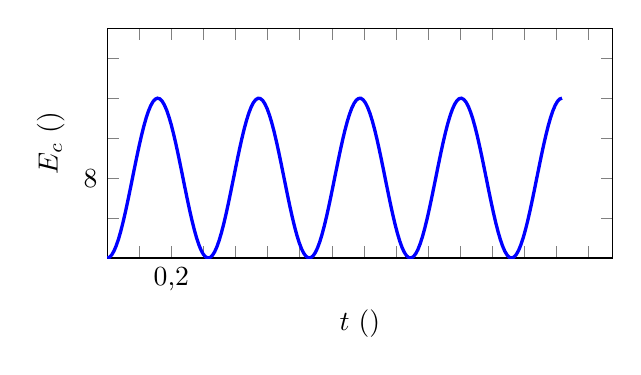
\begin{tikzpicture}
                     \def\Xm{0.04}
                     \def\T{0.63}
                     \def\K{20}
                     \pgfmathpi\let\pi=\pgfmathresult
                     \begin{axis}[
                             xmin=0,xmax=2.5*\T,
                             ymin=0,ymax=23,
                             width=8cm,height=4.5cm,
                             trig format plots=rad,
                             xtick distance=0.1, ytick distance=4,
                             xticklabels={,,,{0,2}}, yticklabels={,,,8},
                             xlabel=$t~(\unit{\second})$,
                             ylabel=$E_{c}~(\unit{\mJ})$,
                             minor tick num=0,
                         ]
                         \addplot[domain=0:2.25*\T,samples=200,very thick,blue]
                             {0.5*\K*\Xm*\Xm*sin(2*pi/\T*x)*sin(2*pi/\T*x)*1e3};
                     \end{axis}
                 \end{tikzpicture}
                 \caption{}
                 \label{fig:Ec_de_t}
              \end{figure}   
          \end{minipage}
\end{enumerate}

